\section{Dataset \& Features}

%  "download data"
\textbf{(1) Download Raw Data:} The raw data is downloaded from the Mecklenburg
County ArcGIS Sales platform, providing a .csv file containing property sales
data. The dataset includes various features, as outlined in Table 1.
\begin{table}[h!]
	\centering
	\caption{Features in the Raw Data}
	\renewcommand{\arraystretch}{1} % Reduce row height
	\setlength{\tabcolsep}{8pt} % Reduce column padding
	\begin{tabular}{|l|l|l|l|l|l|l|l|}
		\hline
		\texttt{parcelid}   & \texttt{transferid} & \texttt{propertyid} & \texttt{saleprice} & \texttt{saledate} & \texttt{soldasvaca} & \texttt{landuseful}  & \texttt{landuse}     \\
		\hline
		\texttt{deeddescri} & \texttt{legalrefer} & \texttt{salesvalid} & \texttt{naldesc}   & \texttt{grantor}  & \texttt{grantee}    & \texttt{shape\_Leng} & \texttt{shape\_Area} \\
		\hline
	\end{tabular}
\end{table}

% "(2) WebScraping/processArcGISSales.py"
\textbf{(2) Data Cleaning:} A Python script processes the raw data in chunks of
10,000 rows for efficient handling of large data volumes. The cleaning process involves:
(1) dropping rows with missing \texttt{transferid} or \texttt{parcelid}, (2) removing
records with \texttt{saleprice} equal to 0, and (3) discarding columns that are not
required for subsequent analysis.

\textbf{(3) Feature Engineer [Acres]:} The feature \texttt{Acres} is calculated by
converting the raw \texttt{shape\_Area} values from square feet to acres.

\textbf{(4) Feature Engineer [VDL Sale Price]:} The feature \texttt{VDL Sale
Price} is computed by dividing \texttt{saleprice} by the count of records sharing
the same \texttt{transferid}. This adjustment accounts for multiple parcels associated
with a single transaction.

% "(3) TransformData/2_findHomeToLotRatio.py"
\textbf{(5) Feature Engineer [Adjusted Finished Home Value]:} For records with
unique \texttt{Home Transfer ID}, the corresponding Finished Home Value is
divided by the count of properties linked to that ID. This adjustment normalizes
the finished home value for cases involving multiple properties under a single transfer.

\textbf{(6) Feature Engineer [House to Lot Ratio]:} The \texttt{House to Lot
Ratio} is determined by dividing the \texttt{Adjusted Finished Home Value} by
the \texttt{VDL Sale Price}, provided the latter is non-zero.

% "(3) TransformData/3_queryRecordAddress.py"
\textbf{(7) Feature Engineer [Latitude, Longitude]:} The script queries a public
GIS API to retrieve the first address associated with each \texttt{parcelid}. The
Google Geocoding API is then used to derive the geographical coordinates (latitude
and longitude) for parcels with valid addresses.

\begin{minipage}[t]{0.48\textwidth}
	\centering
	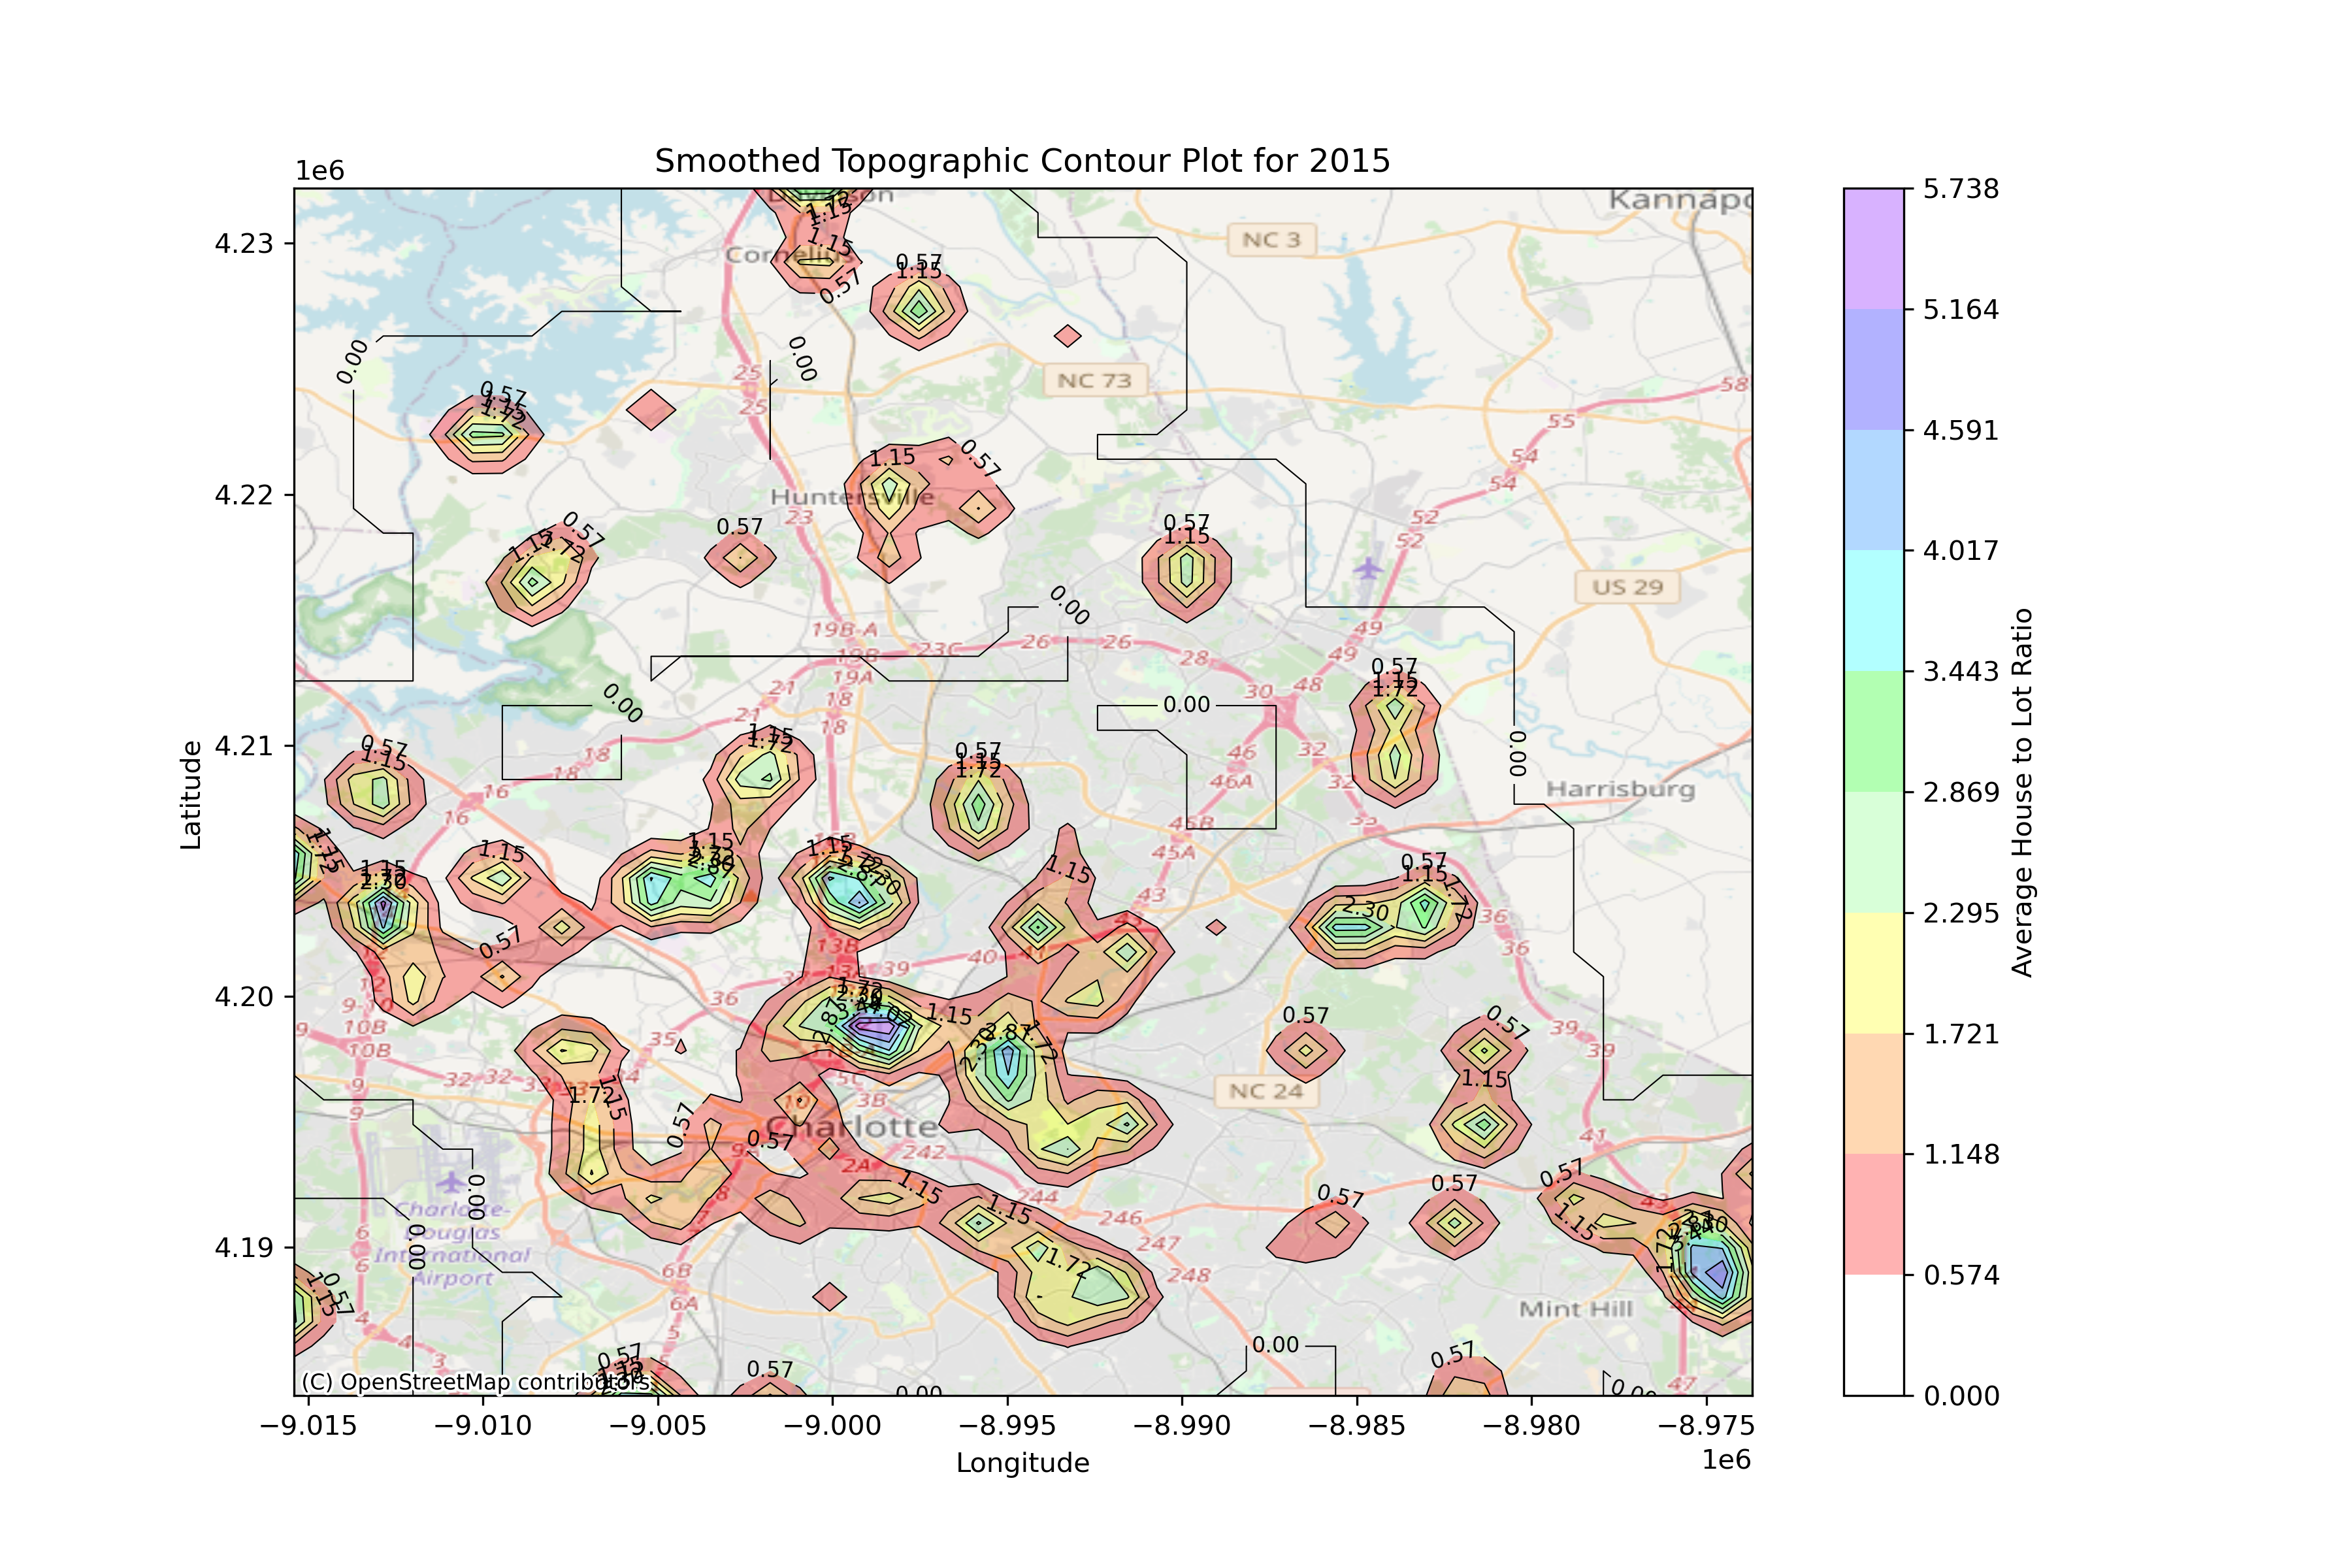
\includegraphics[width=\textwidth]{Sections/House_to_Lot_Ratio_2015.png}
	\captionof{figure}{Visual Mapping of House to Lot Ratio (2015)}
\end{minipage}%
\hfill
\begin{minipage}[t]{0.48\textwidth}
	\centering
	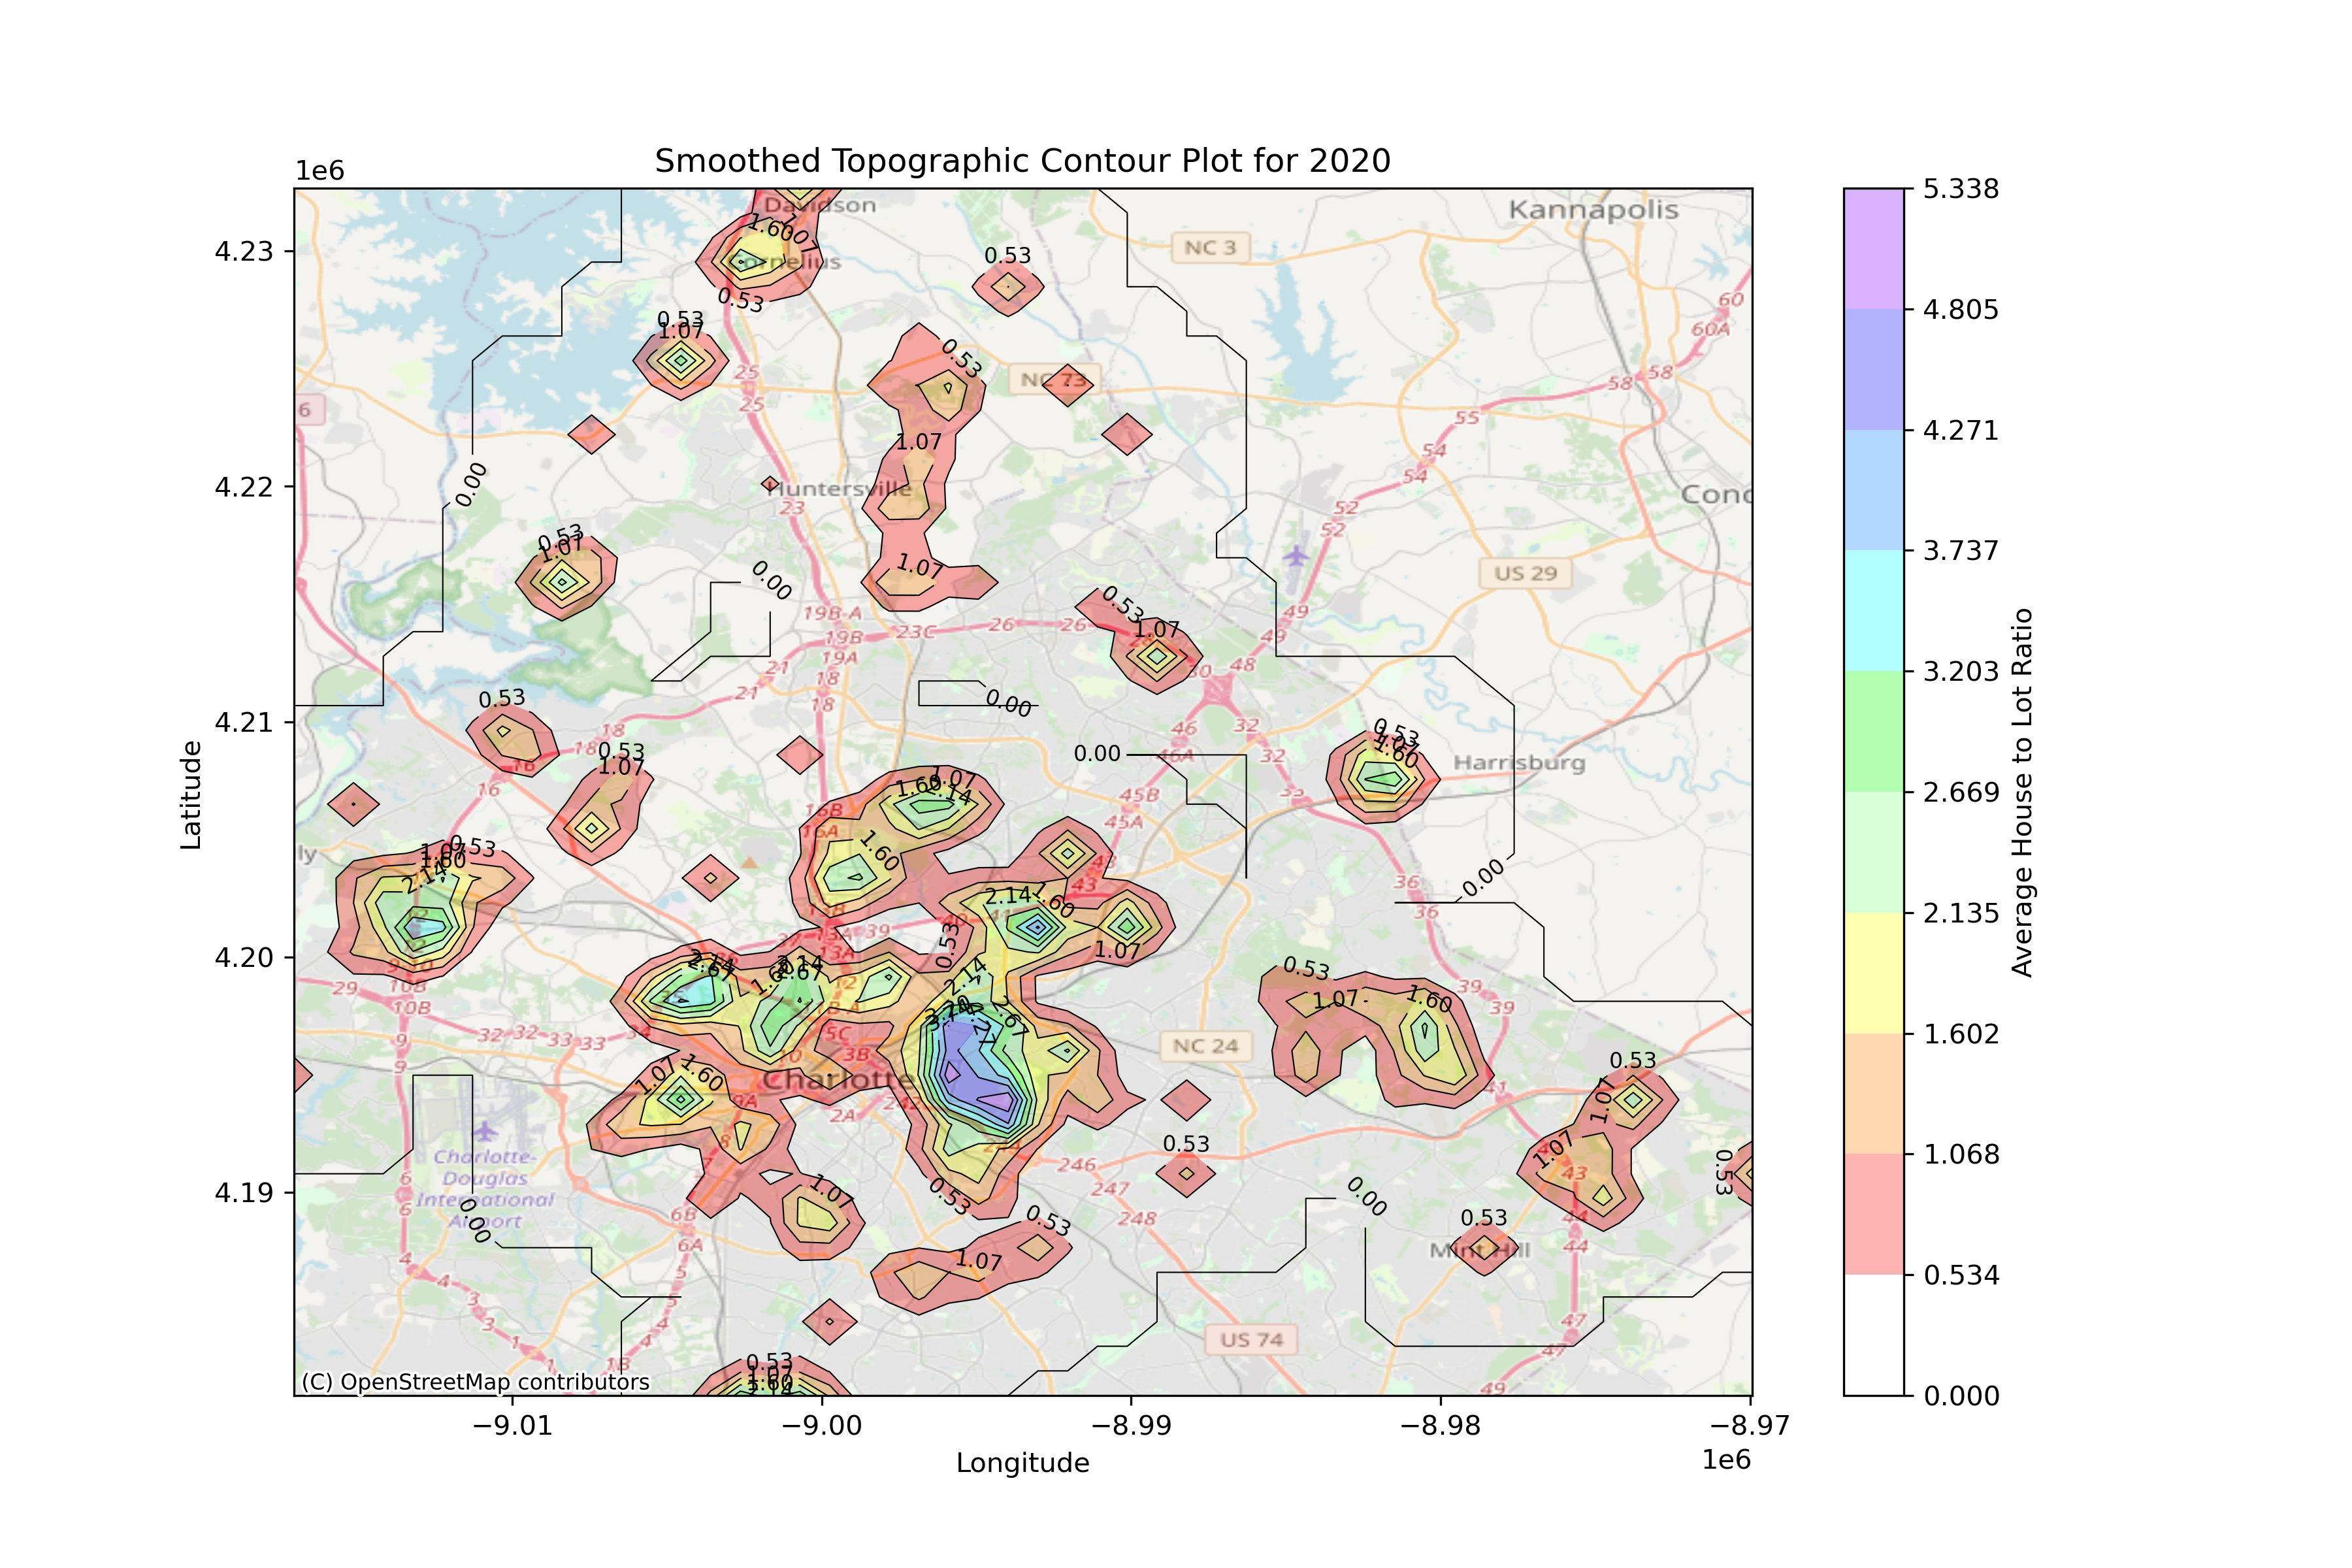
\includegraphics[width=\textwidth]{Sections/House_to_Lot_Ratio_2020.png}
	\captionof{figure}{Visual Mapping of House to Lot Ratio (2020)}
\end{minipage}

% "(3) TransformData/4_addFeatures.py"
\textbf{(8) Feature Modification [Landuse]:} Records are filtered based on a
predefined dictionary of land-use categories, which identifies land-use types to
"keep" or "drop." Only rows with land-use types marked as "keep" are retained. Examples
of "keep" categories are listed in Table 2.
\begin{table}[h!]
	\centering
	\caption{Land Use Features Marked as "Keep"}
	\renewcommand{\arraystretch}{1} % Reduce row height
	\setlength{\tabcolsep}{8pt} % Adjust column padding
	\begin{tabular}{|l|l|}
		\hline
		USE VALUE HOMESITE                  & SINGLE FAMILY RESIDENTIAL              \\
		\hline
		RURAL HOMESITE                      & SINGLE FAMILY RESIDENTIAL - COMMON     \\
		\hline
		SINGLE FAMILY RESIDENTIAL - ACREAGE & MULTI FAMILY GARDEN                    \\
		\hline
		TOWN HOUSE SFR                      & SINGLE FAMILY RESIDENTIAL - WATERFRONT \\
		\hline
		MULTI FAMILY                        & MULTI FAMILY DUPLEX/TRIPLEX            \\
		\hline
		SINGLE FAMILY RESIDENTIAL - GOLF    & MULTI FAMILY MARINA LAND               \\
		\hline
		SCHOOL, COLLEGE, PRIVATE            & SINGLE FAMILY RESIDENTIAL - RIVER      \\
		\hline
	\end{tabular}
\end{table}

% "(3) TransformData/4.23_addStandardizedGranteeNames.py"
\textbf{(9) Feature Engineer [Mapped Grantee]:} The \texttt{Mapped\_Grantee}
column is created by standardizing the \texttt{grantee} names using a dictionary-based
mapping. This eliminates variations in grantee names caused by inconsistent
formats or spellings. Records with grantee values appearing only once are excluded,
focusing on more frequent entities.
\begin{table}[h!]
	\centering
	\caption{Mapping Original Grantee Variations to Standardized Grantee (Example)}
	\renewcommand{\arraystretch}{1} % Adjust row height
	\setlength{\tabcolsep}{8pt} % Adjust column padding
	\begin{tabular}{|l|l|}
		\hline
		\textbf{Standardized Mapped Grantee}   & \textbf{Original Grantee Variations} \\
		\hline
		\multirow{4}{*}{D R HORTON-REGENT LLC} & D R HORTON INC                       \\
		                                       & D R HORTON REGENT LLC                \\
		                                       & D R HORTON                           \\
		                                       & D R HORTON INC                       \\
		\hline
	\end{tabular}
\end{table}

% "(3) TransformData/4.24_transformData.py"
\textbf{(10) Feature Modification [Saledate]:} The \texttt{saledate} column is
reformatted into a \texttt{YYYY-MM} format for consistency and ease of time-series
analysis.

% "(3) TransformData/4.25_findBestIQRGrid.py" "(3) TransformedData/4.26_transformData_BestIQRHypTuning.py"
\textbf{(11) Systematically Remove Outliers Using Inner Quartile Range:} The
script systematically removes outliers by applying IQR thresholds to features
such as \texttt{House to Lot Ratio}, \texttt{Acres}, and \texttt{VDL Sale Price}.
Threshold ranges between [0, 0.2] are tested iteratively, and the dataset is
filtered based on the optimal threshold values that maximize model performance. Outliers
are removed through the following steps: (1) calculate IQR for each feature, (2)
determine the lower and upper bounds using the threshold configuration, (3)
exclude records outside these bounds.
\[
	\begin{aligned}
		Q_{1}      & = \begin{cases}x_{k}&\text{if }n \cdot p \text{ is an integer, where }p = \text{bottom\_range}, \\ x_{\lfloor n \cdot p \rfloor + 1}&\text{otherwise},\end{cases}  \\
		Q_{3}      & = \begin{cases}x_{k}&\text{if }n \cdot p \text{ is an integer, where }p = 1 - \text{top\_range}, \\ x_{\lfloor n \cdot p \rfloor + 1}&\text{otherwise},\end{cases} \\
		\text{IQR} & = Q_{3}- Q_{1}, \quad \text{Lower Bound}= Q_{1}- 1.5 \cdot \text{IQR}, \quad \text{Upper Bound}= Q_{3}+ 1.5 \cdot \text{IQR}.
	\end{aligned}
\]
The model performance is evaluated on each configuration using $R^{2}$ and Mean Squared
Error (MSE). The best-performing thresholds are applied to the final dataset. A summary
of feature ranges and model test results is provided in Table 3 and Table 4,
respectively.
\begin{minipage}[t]{0.48\textwidth}
	\centering
	\captionof{table}{Feature Ranges}
	\renewcommand{\arraystretch}{1} % Adjust row height
	\begin{tabular}{|c|c|c|}
		\hline
		\textbf{Feature Name} & \textbf{Bottom} & \textbf{Top} \\
		\hline
		House to Lot Ratio    & 0.2             & 0.05         \\
		\hline
		Acres                 & 0.15            & 0.2          \\
		\hline
		VDL Sale Price        & 0.15            & 0.2          \\
		\hline
	\end{tabular}
\end{minipage}%
\hfill
\begin{minipage}[t]{0.48\textwidth}
	\centering
	\captionof{table}{Model Test Results}
	\renewcommand{\arraystretch}{1} % Adjust row height
	\begin{tabular}{|c|c|}
		\hline
		\textbf{Metric} & \textbf{Value} \\
		\hline
		Records Used    & 14735          \\
		\hline
		$R^{2}$ Test    & 0.903          \\
		\hline
		MSE Test        & 19.850         \\
		\hline
	\end{tabular}
\end{minipage}

The following section presents statistical summaries and distribution graphs for
the dataset, providing a visual and numerical overview of key features. These insights
help to highlight patterns, trends, and potential anomalies, forming the
foundation for subsequent analysis and model development.

\begin{minipage}[t]{0.3\textwidth}
	\centering
	\includegraphics[width=\linewidth]{
		Sections/ratio_distribution.png
	} % Replace with your image file
	\captionof{figure}{Feature Distribution: [Ratio]} % Caption for the second image
\end{minipage}%
\hfill
\begin{minipage}[t]{0.3\textwidth}
	\centering
	\includegraphics[width=\linewidth]{
		Sections/acre_distribution.png
	} % Replace with your image file
	\captionof{figure}{Feature Distribution: [Acre]} % Caption for the third image
\end{minipage}

The distributions of the data are not weighted uniformly, indicating potential imbalances
or biases in the dataset. This uneven distribution will need to be carefully
addressed during model development to ensure accurate and reliable predictions.

% "(3) TransformedData/4.26_transformData_BestIQRHypTuning.py"